
\section{ Linear regresion }
\subsection{Stochastic gradient descendent}


Stochastic gradient descendent (SGD) is a sequential version of the gradient descent. Instead of considering the full batch gradient on all $N$
training data points, we condider a stochastic version of the gradient. Firts, pick a training data point $(x_n, y_n)$ uniformly random
(hence the name 'stochastic') and consider only the error on that data point.  \cite{LFD}

The gradient of this single data point's error is used for the weight update in exactly the same that the gradient was used in batch gradient descent.

Another variants are the \textbf{mini-batch gradient descent} and the \textbf{batch gradient descendent}, the differences among them are the size of the batch: one for the pure stochastic gradient descendent, between 32 or 64 for the mini-batch variation and more than that for the batch gradient descendent.


\subsection{Pseudo - inverse algorithm}
Pseudo inverse algorithm also known as \textbf{linear regression algorithm} or \textbf{ordinary least squares}(OLS) is based on minimizing the squared error between the 
proyection matrix $h(x) = w^T x$ and $y$, the target vector, where $x \in \mathbb R^{N \times (d+1)}$ is the feature matrix and
$N \in \mathbb N$ the training data size.   

\begin{equation*}
  E_{in}(w) = \frac{1}{N} \sum_{n=1}{N} (w^T x_n - y)^2 
  = \frac{1}{N} \| Xw -y \|^2 
\end{equation*}

Where $\|.\|$ is the Euclidean norm of a vector.

Since $E_{in}(w)$ is differenciable we can use standard matrix calculus to find the $w$ that minimizes  $E_{in}$ with respect to w is the zero vector:

$$\nabla E_{in}(w) = \frac{2}{N}(X^TXw - X^T y) =0$$
Finally to get $\nabla  E_{in}(w)$ to be $0$, one should solve for $w$ that satisfies

$$X^TXw = X^y$$

If $X^TX$ is invertible, $w = X^\dagger y$ where $X^\dagger = (X^T X)^{-1}$ is the \texttt{pseudo-inverse} of $X$. The resulting $w$ is the unique optimal solution that minimizes $E_{in}$.  Otherwise a pseudo-inverse can still be defined, but the solution will not be unique.

In practice, $X^TX$ is invertible in most of the cases since $N$ is often much bigger than $d+1$, so there wil likely be $d+1$ linerly indepent vector $x_n$.



\subsection{Exercise 1}

Estimate a linear regression model from the data provided by the
feature vectors (Average intensity, Symmetry)
using both the pseudo-inverse algorithm and the Stochastic Gradient Descent (SGD).
The labels will be $\{-1,1\}$,
one for each feature vector of each number.
Draw the solutions obtained together with the data used in the fitting.
Assess the goodness of the result using Ein and Eout
(for Eout calculate the predictions using the data from the test file).



\subsubsection{Error}


As we have said the error is the mean squared error:
$$E_{out}(h) = \mathbb E [(h(x) -y)^2]$$
 $$E_{in}(w)  = \frac{1}{N} \| Xw -y \|^2$$

A direct implementation is

\begin{minted}{python}
  def Error(x,y,w):
    '''quadratic error 
    INPUT
    x: input data matrix
    y: target vector
    w:  vector to 

    OUTPUT
    quadratic error >= 0
    '''
    error_times_n = np.linalg.norm(x.dot(w) - y.reshape(-1,1))**2
  
    return error_times_n/len(x)

  \end{minted}

  

  For the euclidian norm we have used \texttt{np.linalg.norm} \cite{norm} numpy function.

  The gradient computation is direct too:

  $$\nabla E_{in}(w) = \frac{2}{N}(X^TXw - X^T y)= \frac{2}{N}(X^T(Xw -  y))$$
  
\begin{minted}{python}
  def dError(x,y,w):
  ''' gradient
  OUTPUT
  column vector
    '''

    return (2/len(x)*(x.T.dot(x.dot(w) - y.reshape(-1,1))))
  \end{minted}

  \subsubsection{Interpretation of the mean squared error, E}
  The mean squared error funcion $E: \mathbb R ^d \longrightarrow \mathbb R^+_0$ measures the average of the squared difference between the estimated values ant the actual value\cite{MSE}. Hence, the nearer to zero, the better.

  
  

\subsubsection{Pseudo-inverse algorithm}

As we have described in pseudo inverse introduction, firstly we need to compute the pseudo-inverse. For that we have use  \texttt{np.linalg.pinv} \cite{pseudo-inverse}function from numpy library.

\begin{minted}{python}
  def pseudoInverseMatrix ( X ):
    '''
    INPUT 
    X: is a matrix (must be a np.array) to use transpose and dot method
    OUTPUT
    hat matrix 
    '''

    '''
    #S =( X^TX ) ^{-1}
    simetric_inverse = np.linalg.inv( X.T.dot(X) )

    # S X^T = ( X^TX ) ^{-1} X^T
    return simetric_inverse.dot(X.T)
    '''
    return np.linalg.pinv(X)
\end{minted}

Finally we have to compute $w = X^\dagger y$


\begin{minted}{python}
  def pseudoInverse(X, Y):
    ''' 
    INPUT
    X is the feature matrix 
    Y is the target vector (y_1, ..., y_m)
    
    OUTPUT: 
    w: weight vector
    '''
    X_pseudo_inverse = pseudoInverseMatrix ( X )
    Y_transposed = Y.reshape(-1, 1)
    
    w = X_pseudo_inverse.dot( Y_transposed)
    
    return w

  \end{minted}

  \subsubsection{Pseudo-inverse linear regression model}

  After execute the algorithm we obtain:

\begin{verbatim}
___ Goodness of the Pseudo-inverse fit ___

  Ein:   0.07918658628900395
  Eout:  0.1309538372005258

Evaluating output training data set
Input size:  1561
Bad negatives : 7
Bad positives : 3
Accuracy rate : 99.35938500960923 %

Evaluating output test data set
Input size:  424
Bad negatives : 1
Bad positives : 7
Accuracy rate : 98.11320754716981 %

\end{verbatim}

  Which means that the $w$ calcs by our pseudo-inverse algorithm we the training data set has a $E_{in}(w) = 0.079$ and with the test data $E_{out}(w) = 0.131$, for our experiment it is a good fit, because it is close enough to zero. In addition, if we evaluate the data classification,
  from $1561$ traing data it only misclassify $10$, whereof 7 was truely positives. The accuracy rate $(\frac{\text{good classified data}}{\text{data set size}})$
  is $99.358 \%$, which continues being really good.

  Initially, we could think that it classifies the positives values better, but if we analyse the output from test data set, there are more negatives values misclassified, so we cannot stablish any relation. Moreover here the accuracy rate is $98.113 \%$

  Finally, a graphic representation for the solutions is

  
  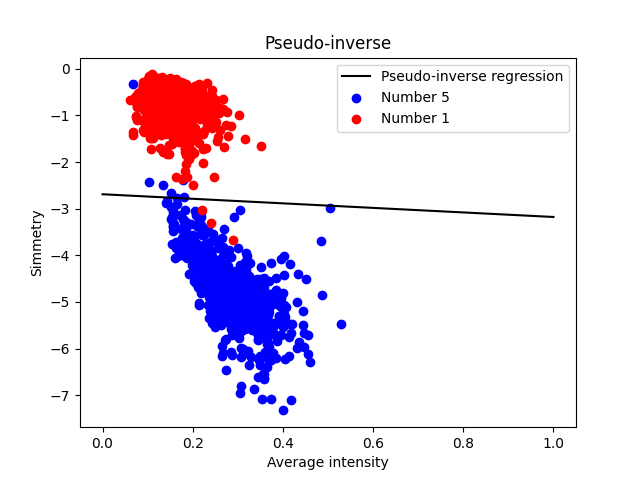
\includegraphics[width=\linewidth]{2_1_pseudo_inverse.png}


  \subsubsection{How have we plotted the regression line.}

  Firstable, to draw a line we need two points.

  Therefore we use the signum to classify the numbers, we are going to find two points in $\mathbb R^2$ that their stimation is zero, which means that they are in the middle of classification (the regression line).

  The obtainied weight vector $w^T = (w_1,w_2,w_3)^T$, means that for a point $(x,y) \in \mathbb R^2$
  its stimation is $h(x,y) = (1,x,y) w = w_1 + w_2x + w_3y$.

  To calcule the two points we are going to equal $h(x,y)=0$ and from the infinities solution we can calculate:

  if $x=0$ then $y = \frac{- w_1}{w_3}$, and if  $x=1$ then $y = \frac{- w_1 - w_2}{w_3}.$
  

  The related code is


  \begin{minted}{python}
    # regression line
    # x= 0
    symmetry_for_cero_intensity = -w[0]/w[2]

    #  x = 1, 0 = w0 + w1 * w2 * x2
    # then y = (-w0 - w1) /w2
    symmetry_for_one_intensity= (-w[0] - w[1])/w[2]

    # plotting order
    plt.plot([0, 1],
             [symmetry_for_cero_intensity,symmetry_for_one_intensity],
             'k-',
             label=(title+ ' regression'))
     
  \end{minted}

  
  
 
\subsubsection{Initial point}  
training data

Motivo de 1, -1 para compensar la etiqueta

HAcer 200

W no importa en la práctica (podemos manipularlo)

VISUALIZAR MODELO CON SCATTER PLOT (DIAPOSITVA 22, CON LOS DATOS ENTRENAMIENTO Y TEST)t

E w deberá de ser la misma

Incluir valor de $E_in E_oit$ y eroro de clasificación (lo normal es que el error en test sea un poquito peor que los de entrenamiento.

Gradiente descendiente minimizar eterativamente:

En el segunto no tiene porqué darse que una iteración sea mejor (otra cosa es que mejore la tendencia mejor)

Si se utilizan todos sí que debería de ir mejorando de manera global.


\subsection{ How to plot }

As we know $w = ( cte, intensity-coeffinient, symmetry-coefficient) = (c,i,s)$ have three parameters. And we are going to plot in a 2D grap where

$c + x i + y s = 0$, it is a line, so we are going to compute two points, the one that x 

$(x = 0): y = frac{-c}{y}$
$(x=1): y = frac{-c - i}{y}$



\section{Experiment }

\subsection{a) Generate a training sample}

We are going to use a uniform generation:

\begin{minted}{python}
def simula_unif(N, d, size):
        ''' generate a trining sample of N  points
in the square [-size,size]x[-size,size]
'''
        return np.random.uniform(-size,size,(N,d))
 
\end{minted}

After fixed radom seed to $1$.

The final 2D map  is

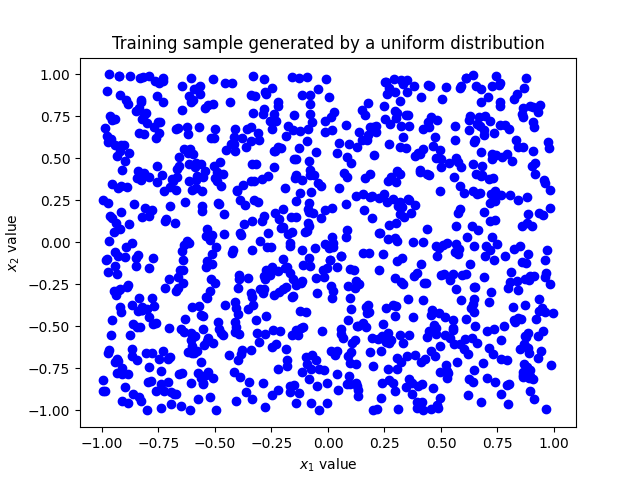
\includegraphics[width=\linewidth]{2_2_a_training_sample.png}

\subsection{b) Labels, noise and map}

b) Let's consider the function $f(x_1, x_2) = sign((x_1 - 0.2)^2 + x_2^2 - 0.6)$ that we will use to assign a label to each point of the previous sample. We introduce noise on the labels, randomly changing the sign of 10 \% of them.
Draw the obtained labels map.


Before plotting, while analysing the function is important to have in mind that a ciercumference with radius $r$ and center $(c_1, c_2) \in \mathbb R^2$ are the points $(x_1, x_2) \in \mathbb R^2$ that verify 

\[ (x_1 - c_1)^2 + (x_2 - c_2)^2 = r^2\]

Therefore looking at $f$ it is easy to think that we are goint to see a circle of radius $\sqrt{0.6}$ and center $(0.2, 0)$.

The plotting is

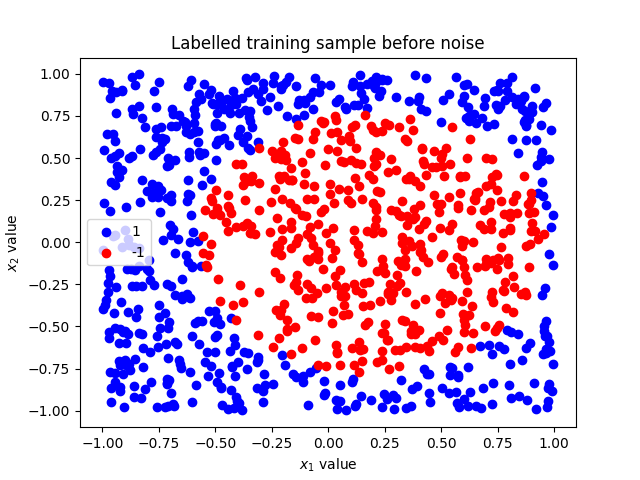
\includegraphics[width=\linewidth]{/2_2_b_labelled_before_noise.png}

In order to introduce noise on the label we are going to change randomly the sign of the $10\%$ of  the labels obtained by $b$.



\begin{minted}{python}
#labels 
y = np.array( [f(x[0],x[1]) for x in training_sample ])

index = list(range(size_training_example))
np.random.shuffle(index)

percent_noisy_data = 10.0
size_noisy_data = int((size_training_example *percent_noisy_data)/ 100 )


noisy_y = np.copy(y)
for i in index[:size_noisy_data]:
    noisy_y[i] *= -1

  \end{minted}

  As we can see the idea behind the snippet is simple: The noised labels would be a copy of the original one and $10\%$ of the data would change their sign.

  The final map is :


  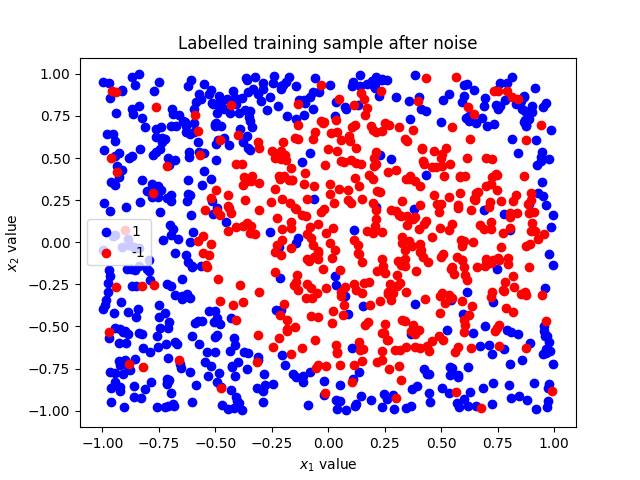
\includegraphics[width=\linewidth]{2_2_b_labelled_after_noise.png}
  

  \subsection{ Estimate the fitting error of $E_{in}$ using SDG}

  c) Using $(1, x_1, x_2)$ as feature vector, fit a linear regression model to the generated dataset and estimate the weights w. Estimate the fitting error of Ein using Stochastic Gradient Descent (SGD).

  Having in mind the observation in the last subsention that the labels follows a circumference equation with a bit of noise, a linear regression model it is not going to be the best approach.

  The experiment result are:
That for a linear SGD with batch size $32$ the $E_{in}$ is   $0.930$

And valuating output training data set
Input size:  1000
Bad negatives : 187
Bad positives : 224
Accuracy rate : 58.9 \%


Remember that the bad negatives are the points that the regression classify in negative but they are positives and the bad positives are the negatives one that are classify as a positives.

Finally the accuracy rate was the corrected classify data divided by the input size, so it is not a good model due to the fact that the accuracy rate is so close to a random one, that it would theoretically have a $50\%$ of a accuracy rate.

A visual representation of de fix is


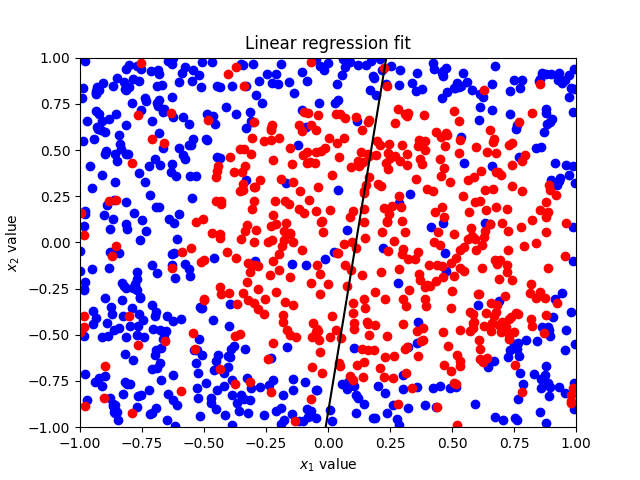
\includegraphics[width=\linewidth]{2_2_c_linear_regression.png}





execution:
\begin{verbatim}
>>> _______LINEAR REGRESSION EXERCISE _______

Exercise 1


 Enter to start


___ Goodness of the Stochastic Gradient Descendt (SGD) fit ___


	SGD, batch size 2
Ein:  0.0822091904727966
Eout:  0.13268719301475448

Evaluating output training data set
Input size:  1561
Bad negatives : 8
Bad positives : 3
Accuracy rate : 99.29532351057014 %

Evaluating output test data set
Input size:  424
Bad negatives : 1
Bad positives : 7
Accuracy rate : 98.11320754716981 %

	SGD, batch size 32
Ein:  0.08145689246982911
Eout:  0.13524833395770525

Evaluating output training data set
Input size:  1561
Bad negatives : 6
Bad positives : 3
Accuracy rate : 99.4234465086483 %

Evaluating output test data set
Input size:  424
Bad negatives : 1
Bad positives : 7
Accuracy rate : 98.11320754716981 %

	SGD, batch size 200
Ein:  0.0815451181277193
Eout:  0.13602151565370962

Evaluating output training data set
Input size:  1561
Bad negatives : 6
Bad positives : 3
Accuracy rate : 99.4234465086483 %

Evaluating output test data set
Input size:  424
Bad negatives : 1
Bad positives : 7
Accuracy rate : 98.11320754716981 %

	SGD, batch size 15000
Ein:  0.08144533934205953
Eout:  0.13486901151111522

Evaluating output training data set
Input size:  1561
Bad negatives : 7
Bad positives : 3
Accuracy rate : 99.35938500960923 %

Evaluating output test data set
Input size:  424
Bad negatives : 1
Bad positives : 7
Accuracy rate : 98.11320754716981 %

___ Goodness of the Pseudo-inverse fit ___

  Ein:   0.07918658628900395
  Eout:  0.1309538372005258

Evaluating output training data set
Input size:  1561
Bad negatives : 7
Bad positives : 3
Accuracy rate : 99.35938500960923 %

Evaluating output test data set
Input size:  424
Bad negatives : 1
Bad positives : 7
Accuracy rate : 98.11320754716981 %

--- Type any key to continue ---
º
Exercise 2


EXPERIMENT (a) 


EXPERIMENT (b) 


EXPERIMENT (c) 


	SGD, batch size 32
Ein:  0.9301633062413852

Evaluating output training data set
Input size:  1000
Bad negatives : 187
Bad positives : 224
Accuracy rate : 58.9 %

 EXPERIMENT (d), lineal regression

The mean value of E_in in all 1000 experiments is: 0.0009131004444134428
The mean value of E_out in all 1000 experiments is: 0.000905505366572186

EXPERIMENT (e)


For one experiment:

 SGD, batch size 32
Ein:  0.6158558061444251

Evaluating output training data set
Input size:  1000
Bad negatives : 88
Bad positives : 50
Accuracy rate : 86.2 %

The mean value of E_in in all 1000 experiments is: 0.0003827441225550457
The mean value of E_out in all 1000 experiments is: 0.00037845910961602556
>>> 

\end{verbatim}